\documentclass[12pt,letterpaper]{article}
\usepackage[latin1]{inputenc}
\usepackage[english]{babel}
\usepackage{amsmath}
\usepackage{amsfonts}
\usepackage{amssymb}
\usepackage{graphicx}
\usepackage{geometry}
\usepackage{enumerate}
\usepackage{verbatim}
\usepackage{subfig}
\usepackage{url}
\geometry{verbose,letterpaper,tmargin=4cm,bmargin=3cm,lmargin=3cm,rmargin=3cm}


%%%%%%% New Commands %%%%%%%%%
\newcommand{\pardiff}[2]{\frac{\partial #1}{\partial #2}}

%%%%%%%%%%%%%%%%%%%%%%%%%%%%%%

\author{Nicol\'as Guar\'in Zapata}
\title{\textbf{Elastic waves}}

\begin{document}
\maketitle

% Introduction about waves in general
\section{Introduction}
A wave is the propagation of certain medium property perturbation, e.g., density, pressure, electric field or magnetic field, that travel through the space transporting energy. The perturbed medium could be of diverse nature like air, water, a piece of metal or vacuum.

The property that presents the phenomena is expressed as function of position and time $\psi(\vec{r},t)$. Mathematically  it is said that $\psi$ is a wave if it verifies the wave equation:
\[\nabla^2 \psi(\vec{r},t)= \frac{1}{v^2} \frac{\partial^2 }{\partial t^2}\psi(\vec{r},t) \enspace ,\]
where $v$ is the wave propagation speed. For instance, some perturbations of the pressure, called sound, verify the above equation, although some non-linear equations have undulatory solutions, e.g., a soliton. 

\subsection{Wave characteristics}
There are great variety of waves but all of them could experiment
\begin{itemize}
\item \textbf{Reflection}:Occurs when a wave find a new medium, that can not cross, change its direction.

\item \textbf{Refraction}: Occurs when a wave change its direction when enter in a new medium with different propagation speed.

\item \textbf{Doppler Effect}: Effect caused by the relative motion between the source and the receptor.

\item \textbf{Interference}: Occurs when two or more waves coexist in the same place and are superimposed.

\item \textbf{Diffraction}: Occurs when a wave find the border of an obstacle and change its \emph{form} to round it.
\end{itemize}


% The most simple case, waves in a string
\section{Waves in a string}
For a string with length $L$, linear mass density $\lambda$ and a tension $T$, let's take a small segment with small displacements in $y$. The force balance over the element showed in Figure 1 is:
\begin{align*}
F_y &= T \sin(\theta + \Delta \theta) - T \sin(\theta)\\
F_x &= T \cos(\theta + \Delta \theta) - T \cos(\theta) \enspace ,
\end{align*}
due to the small displacements the angles are also small and then
\begin{align*}
F_y &\approx T (\theta + \Delta \theta) - T (\theta) = T \Delta \theta\\
F_x &\approx 0 \enspace .
\end{align*}

\begin{figure}[h]
\centering
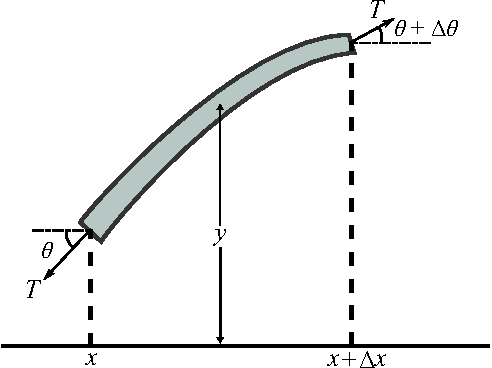
\includegraphics[height=6cm]{img/string.pdf}
\caption{Forces diagram over an element of the string with length $\Delta x$. }
\end{figure}

From the second Newton's law we get
\[T\ \Delta \theta = \underbrace{(\lambda\ \Delta x)}_\text{mass} a_y \enspace ,\]
if we take the limit $\Delta x \rightarrow dx$
\begin{equation}
T\ d\theta = (\lambda\ dx) a_y \enspace .
\label{eq:stringForce}
\end{equation}
And we know that $\tan \theta = \frac{\partial y}{\partial x}$, taking derivative respect $x$
\[\sec^2 \theta \frac{d\theta}{dx} = \frac{\partial^2 y}{\partial x^2} \enspace .\]
Due to small displacements $\sec^2 \theta \approx 1$, hence
\begin{equation}
d\theta \approx \frac{\partial^2 y}{\partial x^2} dx
\label{eq:stringDtheta}
\end{equation}
and replacing (\ref{eq:stringDtheta}) in  (\ref{eq:stringForce})
\[T \frac{\partial^2 y}{\partial x^2} dx = (\lambda\ dx) \frac{\partial^2 y}{\partial t^2} \enspace ,\]
we finally get the 1D Wave Equation
\[\frac{\partial^2 y}{\partial x^2} = \frac{\lambda}{T} \frac{\partial^2 y}{\partial t^2} \enspace .\]

$T/\lambda$ have square speed units, and is the square propagation speed
\[v = \sqrt{\frac{T}{\lambda}} \enspace ,\]
so
\[\frac{\partial^2 y}{\partial x^2} = \frac{1}{v^2} \frac{\partial^2 y}{\partial t^2} \enspace .\]

\subsection{Solution}
The wave equation could be solved by separation of variables, i.e., let's suppose it has a solution of the form $y=y(x,t)=X(x)T(t)=X\ T$
\[\frac{1}{X} \frac{d^2 X}{dx^2} - \frac{1}{v^2 T} \frac{d^2 T}{dt^2} = 0 \enspace ;\]
we can see that the temporal and the spatial terms are isolated, so they should be equal to a constant. For simplicity let's take $-\alpha^2$, with $\alpha\in \mathbb{R}$
\[\frac{d^2 X}{dx^2}=-\alpha^2 X, \qquad \frac{d^2 T}{dt^2}=-\alpha^2 v^2 T \enspace ,\]
so the solution is
\[y = \left[C_1 \sin(\alpha x)+ C_2\cos(\alpha x) \right] \left[C_3\sin(\alpha v t) +C_4 \cos(\alpha v t)\right] \enspace .\]
If we take fixed extremes and assume that the string starts with a deformed shape $f(x)$, i.e., $y(0,t)=y(L,t)$, $y(x,0)=f(x)$ and $y'(x,0)=0$ can be shown that the complete solution is
\[y(x,t) = \frac{2}{L}\sum\limits_{n=1}^{\infty}\left[\int\limits_{0}^{L}f(\xi)\sin\left(\frac{n\pi\xi}{L}\right)d\xi\right] \sin\left(\frac{n\pi x}{L}\right)\cos\left(\frac{n\pi v t}{L}\right) \enspace .\] 

\section{Elastic waves}
In a three dimensional solid we can also describe waves starting from the continuity equation, motion equations and constitutive relationships.\footnote{Here the so called Einstein notation for summations is used, when an index appears twice indicates a summation over the repeated one.}
\begin{itemize}
\item Continuity:
\[\frac{\partial}{\partial t}\rho = - \frac{\partial}{\partial x_i}\left( \rho \frac{\partial}{\partial t} u_i\right)\]

\item Motion equations:
\[ \frac{\partial^2}{\partial t^2}(\rho u_i) = \frac{\partial}{\partial x_j} \sigma_{ij} + f_i \]

\item Constitutive relationships:
\[\sigma_{ij} = C_{ijkl} \epsilon_{kl}  \enspace ,\]

\end{itemize}
where $u_i$ is the displacement of a material point in $i$ direction, $\rho$ is the volume density, $\sigma_{ij}$ the stress tensor, $\epsilon_{kl}$ is the strain tensor, $f_i$ are \emph{body forces}\footnote{Body forces are forces distributed within the volume like gravitational or electromagnetic forces.} and $C_{ijkl}$ depends on the material of the medium.

For an isotropic medium the constitutive relation can be expressed as
\[\sigma_{ij} = \lambda \delta_{ij}\epsilon_{kk} + 2\mu \epsilon_{ij} \enspace ,\]
being $\lambda$ and $\mu$ the Lame parameters.

$\epsilon_{ij}$ is usually define as
\[\epsilon_{ij} = \frac{1}{2} \left( \pardiff{u_i}{x_j} + \pardiff{u_j}{x_i} \right) \enspace ,\]
so
\[\sigma_{ij} = \lambda \delta_{ij} \pardiff{u_k}{x_k} + \mu \left( \pardiff{u_i}{x_j} + \pardiff{u_j}{x_i} \right) \enspace .\]

If we take the constitutive equation and replace $\sigma_{ij}$ in the motion equation (assuming that $\pardiff{\rho}{t}=0$).
\[\rho \pardiff{u_i}{t} = \delta_{ij} \lambda \pardiff{\epsilon_{kk}}{x_j} + 2\mu \pardiff{\epsilon_{ij}}{x_j} +f_i \enspace ,\]
and rewriting the right hand side in terms of the displacements we have
\[\rho \pardiff{^2 u_i}{t^2} = \delta_{ij} \lambda \pardiff{}{x_j}\left( \pardiff{u_k}{x_k}\right) + \mu \pardiff{ }{x_j}\left( \pardiff{u_i}{x_j} + \pardiff{u_j}{x_i}\right) + f_i \enspace ,\]
operating the Kronecker's delta
\[\rho \pardiff{^2 u_i}{t^2} = \lambda \pardiff{}{x_i}\left( \pardiff{u_k}{x_k}\right) + \mu \pardiff{}{x_j}\left( \pardiff{u_i}{x_j} + \pardiff{u_j}{x_i} \right) + f_i \enspace ,\]
and this can be rewritten like
\[\rho \pardiff{^2 u_i}{t^2} = \lambda  \pardiff{^2 u_j}{x_i x_j} + \mu \pardiff{^2 u_i}{x_j^2} + \mu \pardiff{^2 u_j}{x_j x_i} + f_i \enspace ,\]
grouping terms
\begin{equation}
\rho \pardiff{^2 u_i}{t^2} = (\lambda + \mu)  \pardiff{}{x_i}\left( \pardiff{u_j}{x_j} \right) + \mu \pardiff{^2 u_i}{x_j^2}  + f_i \enspace .
\label{eq:navierInd}
\end{equation}
This is the Navier Equation that can be expressed also in vector form
\[\rho \pardiff{^2 u_i}{t^2} = (\lambda + \mu)  \underbrace{\pardiff{}{x_i}}_{\mbox{grad}}\nabla \cdot \vec{u} + \mu \nabla^2 u_i + f_i \enspace ,\]
or
\begin{equation}
\rho \pardiff{^2 \vec{u}}{t^2} = (\lambda + \mu)  \nabla (\nabla\cdot \vec{u})+ \mu \nabla^2 \vec{u} + \vec{f} \enspace .
\label{eq:navierVec}
\end{equation}
The body forces will be neglected hereinafter for simplicity. The vector identity is used
\[\nabla^2 \vec{a} = \nabla (\nabla \cdot \vec{a}) - \nabla \times (\nabla \times \vec{a})\]
and we get
\[\rho \pardiff{^2 \vec{u}}{t^2} = (\lambda + 2\mu) \nabla(\nabla \cdot \vec{u}) - \mu (\nabla \times (\nabla \times \vec{u})) \enspace .\]
If we take $\varphi = \nabla \cdot \vec{u} $ and $\vec{\psi} = \nabla \times \vec{u}$:\footnote{This identity is the Helmholtz Theorem and establish that a vector field can be expressed in terms of vector and scalar potentials. For a deeper description see \cite{book:arfken} page 95.}
\begin{equation}
\rho \pardiff{^2 \vec{u}}{t^2} = (\lambda + 2\mu) \nabla \varphi - \mu \nabla \times \vec{\psi} \enspace .
\label{eq:waveHelm}
\end{equation}

\subsection{P-waves equation}
Taking divergence to (\ref{eq:waveHelm})
\[\nabla\cdot \left( \pardiff{^2 \vec{u}}{t^2} \right)= (\lambda +2\mu) \nabla\cdot \nabla \varphi - \mu\nabla\cdot\nabla\times \vec{\psi} \enspace , \]
we finally get
\begin{equation}
\nabla^2 \varphi = \frac{1}{\frac{\lambda + 2\mu}{\rho}} \pardiff{^2 \varphi}{t^2} \enspace ,
\label{eq:pWave}
\end{equation}
with speed of propagation
\[v_P := \sqrt{\frac{\lambda + 2\mu}{\rho}}\]

\subsection{S-waves equation}
Taking rotational to (\ref{eq:waveHelm})
\[\nabla\times \left( \pardiff{^2 \vec{u}}{t^2} \right)= (\lambda +2\mu) \nabla\times \nabla \varphi - \mu\nabla\times\nabla\times \vec{\psi} \enspace , \]
we finally get
\begin{equation}
\nabla^2 \vec{\psi} = \frac{1}{\frac{\mu}{\rho}} \pardiff{^2 \vec{\psi}}{t^2} \enspace ,
\label{eq:SWave}
\end{equation}
with speed of propagation
\[v_S := \sqrt{\frac{\mu}{\rho}}\]

\section{Summary}

Navier Equation wave behaviour has been proved using Helmholtz potentials, i.e., decomposing the vector field in rotational and solenoidal parts. This decomposition leads to the well known P and S waves, very common in seismology. The names P and S  obey the \emph{Pressure} and \emph{Shear} properties of the waves, respectively. Since $\lambda$ and $\mu$ are positive numbers the $v_P$ is always higher than $v_S$.

Although body forces have been neglected the procedure presented could be used with this kind of forces, in the latter a Helmholtz decomposition has to be done for the body forces in order to handle the P and S waves in a separate manner. In the case of gravitational field the term would be completely solenoidal, and for electromagnetic fields could have rotational and solenoidal parts. Taking the whole Navier equation avoid the decomposition and the body forces could be taken complete.
\pagebreak

\begin{thebibliography}{99}
\bibitem{book:waves-rays} Michael A. Slawinski. Waves and rays in Elastic Continua. Second Edition, 2007.
 
\bibitem{wiki:ondas} Wikipedia community. Onda (f\'isica) [on line]. Wikipedia, La enciclopedia libre, 2010 ; 22 November 2010. Available from \url{<http://es.wikipedia.org/w/index.php?title=Onda_(f%C3%ADsica)&oldid=41971511>}. 

\bibitem{book:arfken} George B. Arfken \& Hans. J. Weber. Mathematical Methods for Physicists. Elsevier Academic Press, 6th Edition, San Diego, 2005.
\end{thebibliography}


\end{document}